%4.2	Alternativas de diseño 
%Describir alternativas de diseño consideradas y las razones usadas para elegir la alternativa finalmente escogida.
\section{Design Alternatives}
%Guante & Flystick & Voice Recognition
%3D Joystick ->2D Joystick + Slider
The goal of this section is to explain the design alternatives and the reasons behind the selection of the alternative that was ultimately implemented. Even in the case that there weren't alternatives at all, like in the system architecture, this section will still explain the pros and cons of the default design.
\subsection{System Architecture}
The system running the application is a three-layered system, as can bee seen in the image below . The top level, the VRPN Tracking servers receives tracking information from the tablet VRPN device, which design will be discussed later, and from the IR tracking cameras following the flat passive markers attached to the back of the tablet.

\begin{center}
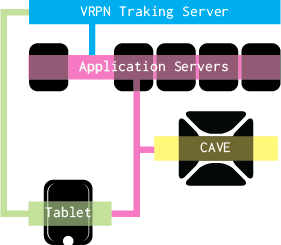
\includegraphics[scale=0.75]{Images/architecture.png}
\label{fig:architecture}
\end{center}

The VRPN server centralizes and retransmits the information from all the interaction devices that interact with the immersive system in which are used, in this case the tablet and the passive stereo glasses. The use of VRPN was a must for the project, as shown by the Non Functional Requirements in the previous chapter. VRPN stands for \emph{Virtual Reality Peripheral Network} and is ``... a set of classes within a library and a set of servers that implement a device-independent, network-transparent interface between application programs and the set of physical devices (trackers, buttons, etc.) used in a virtual reality (VR) system'' as defined by its creators in \cite{vrpn}. The use of VRPN is a development standard at the Institute Image as well as at the COLIVRI laboratory because of the flexibility provided by an abstraction layer that separates front-end devices from the application input.

The second layer is composed by the Application Servers in charge of rendering the scene to project it in the Cave. One of these application servers render the scene from the tablet point of view, and stream the scene in real time, to allow the camera metaphor that will be explained in the User Interaction section of this chapter. Is important to note, that there isn't communication between those servers; each one, renders the scene from a particular perspective calculating the adequate frustrum for it's designated screen. Each of the Application Servers renders the images for both eyes of it's screen, but each image is projected by a different projector in order to work as a passive 3D system.
\subsection{User Interaction}

\subsubsection{Front-end Devices}
There were several initial options for the user interaction design at the start of the project due to the devices already at use at the Institute. Here I'll discuss the reason for choosing an Android tablet over tracking gloves, flysticks and speech recognition. The general principles I took in account to take the decision were the {\emph compatibility} and ease of use of the devices and, when possible, the reduction of the number of front-end devices to the minimum necessary to successfully perform the operations needed to use the application.

The definition of \emph{compatibility between devices} is defined, when the use needs to use two or more devices to interact with the application, as the capability to perform any operation in the system without the need to change a device from hand, or any other action that would increase the interaction complexity. So, two or more devices are incompatible if they can't be used and carried by the user in the same way during the use of the application. For example, if the application uses a flystick to select 3D objects and a glove to allow the user to interact with the application in a gestural way; and the user needs to change the flystick from his left hand to his right hand, because he's right-handed and can't perform precision operations with his left hand \footnote{These factors vary greatly between users, so to broad the validity and applicability of the concept for the purposes of this work, I suppose every user has a dominant hand and can't perform precision operations with his other hand.}, the devices are mutually incompatible under the {\emph interaction paradigm} provided.

The \emph{interaction paradigm} is composed by the set of input actions expected to be made by the user to be able to use the application and the interaction metaphors used to enhance and simplify this interaction.

In this order of ideas, the relevant basic actions are selecting objects (whether they are polygons or menu objects) and writing texts \footnote{Is interesting that even a basic pointing device can be used as a text input device, as shown by the screen-keyboard applications available in Mac OS and Windows. Nevertheless, using a non touchscreen pointing device is incredibly slow and would work as a bottleneck in the application workflow.}. The following analysis explains how the selection of front end devices was made. The term ID implies that there's incompatibility between the proposed devices, OK means there's not.

\begin{tabular}{cc|c|c|c|c|l}
\cline{3-4}
& & \multicolumn{2}{|c|}{Text Input Device} \\ \cline{3-4}
& & Speech Recognition & Tablet \\ \cline{1-4}
\multicolumn{1}{|c|}{\multirow{3}{*}{Selection Device}} &
\multicolumn{1}{|c|}{Flystick}& OK & ID     \\ \cline{2-4}
\multicolumn{1}{|c|}{}                        &
\multicolumn{1}{|c|}{Glove} & OK & ID     \\ \cline{2-4}
\multicolumn{1}{|c|}{}                        &
\multicolumn{1}{|c|}{Tablet} & OK & OK \\ \cline{1-4}
\end{tabular}\\

As can be seen the Tablet is the only device that can be used both as a pointer device and as a text input device. There are several ways to use the Tablet as a pointing device, the one selected in this project due to it's usability and \emph{woah factor} is the window, or blank frame, metaphor. 

A first approximation to the window metaphor can be seen in the work by Jung \cite{Jung}. It consists basically of the use of a screen, its position and rotation to show the scene as if the screen frame was blank. An important difference between the work by Jung and this project is that, in his work, he doesn't take in account the relative motion of the user's head and the screen.


\subsubsection{Application Workflow}

The application workflow is straightforward. It consists of the following steps, separated in two stages \emph{Configuration} and \emph{Execution}:

The Configuration steps are:
\begin{enumerate}
\item Update the Annotations XML and the 3D Model to their latests versions. \footnote{It's highly encouraged the use of a folder synchronization software such as Dropbox® or Ubuntu One®, this can automatize this whole step and render it invisible to the final user}.
\item Start the ART Track Toolkit and start the tracking.
\item Start the VRPN Server.
\item Start the Python Server provided with the software, that will send the XML Annotations to the Tablet and start the application on the server side.
\end{enumerate}

The Execution steps are:
\begin{enumerate}
\item Check the tablet is connected to the same LAN as the other computers used by the application.
\item Launch the 3D Annotations application from the tablet.
\item Follow the instructions.
\end{enumerate}

The instructions during the Execution stage are quite simple, compared to the ones in the configuration stage. Even when the purpose of this project is to deliver a highly usable annotation system, the Configuration Stage can not be simplified. On the other hand these steps must be followed only once, while there's no need to shut down the system. The possibility of automatizing the configuration process will be examined in the future work section.

\subsubsection{User Interface}

There's no user interface for the software running in the CAVE servers, so the following content will explain the user interface of the tablet application. \emph{A poster at the end of this document shows the information below graphically.}

Once the user has executed the application the first screen asks for the user name, this name will be used to fill the author field of the annotations made in this execution session. After typing his name, the user will face a progress dialog while the application connects to the Python Server and retrieves the Annotation XML to be used in this session.

Once the system has load the model and the annotations, the user can start to read the annotations made by others or start annotating the model himself. The main screen of the application is a tabbed window with two tabs: Navigation and Annotations. In the Navigation tab the user will be able to navigate the model using two 3D joysticks located at the bottom of the screen, while in the background and filling almost all the screen space a real-time render of the model will be rendered following the window metaphor discussed above. This render is made by one of the computers running the application and send to the tablet wirelessly using the UDP protocol\footnote{Using TCP would slow down the streaming throughput in the sake of guaranteeing the reception of all the frames by the tablet. A missing frame is not a real problem in a streaming context.}. The CAVE will project the scene based on the calculated location information received by the tablet.

The 3D joysticks were thought to be used without capturing the user's gaze. Nevertheless, given that the scene can be seen in the tablet as well, the user can use the system as he want to; whether seeing the screen or the tablet. When the user reaches the place an annotation was made, he will notice so because a semitransparent sphere will be rendered on top of the model, he can tap the tablet screen where the sphere is shown to examine the annotation's contents. 

In a different case, if the user wishes to crate a new annotation, the user can tap the screen. This will prompt the user to select the desired polygons to annotate. After the polygons are selected he will click the \emph{Annotate} button and a dialog will be shown. The dialog will contain a form to be filled with the annotation priority and it's contents. If the user confirm the annotation, tapping the button \emph{Save}, the annotation will be saved by the CAVE computers in the Annotations XML and the user will return to the navigation Tab. 

The other Tab is the Annotations Tab. Here the user can see a list of all the annotations made in the model organized by priority. In the sake of usability, a button called \emph{Create New Annotation} is shown and it's activation will prompt the user to the navigation screen with the instructions of how to make an annotation.

If the user taps on any of the annotations shown, a dialog with it's details will be shown giving also the option to navigate to the annotation's location. The user can also delete the annotation or return to the Annotations List.
\subsection{Software}
\subsubsection{Cave}
The code used to load and display the model and communicate to the VRPN Server is largely based on the code used by Phillipe which is based on the code developed by Sébastien Guerin. This reuse of code lead to a considerable saving of time and also helped to avoid most of the problems associated with my lack of experience using C++ and OpenScneGraph.

The application running in all the CAVE servers is the exactly the same. The expected differences on behavior and point of view are derived from a configuration file located in the same directory as the executable application. This configuration file facility was already developed in the code authored by Sébastien.

UML
\subsubsection{Tablet}
